
\begin{figure}[ht]
	\centering
	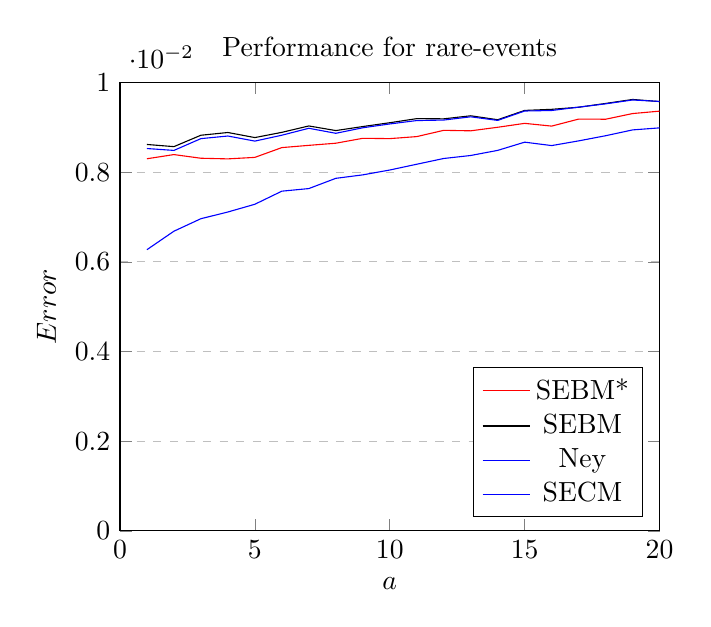
\begin{tikzpicture}[scale=1.0]
		\begin{axis}[
			title={Performance for rare-events},
			xlabel={$a$},
			xmin=0, xmax=20,
			ymin=0.000, ymax=0.01,
			ymajorgrids=true,
			ylabel={$Error$},
			grid style=dashed,
			xticklabel style={/pgf/number format/fixed},
			legend pos=south east,
		]
		\addplot[color=red] coordinates {
		(1,0.00829898628225)(2,0.00839191742155)(3,0.00831034375718)(4,0.00829616185199)(5,0.00832950631521)(6,0.00854788207454)(7,0.00859788647386)(8,0.00864539507562)(9,0.00875494343606)(10,0.00874804130022)(11,0.00879320206649)(12,0.00893286726698)(13,0.00892212687259)(14,0.00900143434975)(15,0.00908826041694)(16,0.00902723165099)(17,0.00918368988491)(18,0.00918072508884)(19,0.00930705761444)(20,0.00936085652527)
		};
\addlegendentry{SEBM*}
		\addplot[] coordinates {
		(1,0.00861758612646)(2,0.00856931333511)(3,0.00882336193996)(4,0.00888456557868)(5,0.00877127203762)(6,0.00888791399471)(7,0.00903070521197)(8,0.00892750294613)(9,0.00901735865911)(10,0.00910237180572)(11,0.00919387192857)(12,0.00918944397918)(13,0.00925732316038)(14,0.00916931563909)(15,0.00937697513676)(16,0.00940154091917)(17,0.00944782712404)(18,0.00953263660509)(19,0.00962165024385)(20,0.00957429275453)
		};
\addlegendentry{SEBM}
		\addplot[color=blue] coordinates {
		(1,0.00627042393191)(2,0.00668283560602)(3,0.00696175803194)(4,0.00711122084588)(5,0.00728404764124)(6,0.00757582039795)(7,0.00763393965732)(8,0.00786227870242)(9,0.00793950292667)(10,0.00804775959656)(11,0.00817661699722)(12,0.00830499867171)(13,0.00837197170234)(14,0.00848570355671)(15,0.00866904091263)(16,0.00859262838231)(17,0.00869764757103)(18,0.00881244467649)(19,0.00894236872475)(20,0.00898769050537)
		};
\addlegendentry{Ney}
		\addplot[color=blue] coordinates {
		(1,0.00852711828901)(2,0.00848494072214)(3,0.00874773654002)(4,0.00880609825734)(5,0.00869268282241)(6,0.00882394889482)(7,0.00897875778344)(8,0.0088667004212)(9,0.0089897364589)(10,0.00907540185807)(11,0.00915081153869)(12,0.00916218423184)(13,0.0092344860602)(14,0.00915425878397)(15,0.00936396139817)(16,0.00937527442835)(17,0.00945006806042)(18,0.00952384116565)(19,0.0096100208579)(20,0.00957776196452)
		};
\addlegendentry{SECM}
		\end{axis}
	\end{tikzpicture}
    \caption{Average error of three stratified random sampling methods for the uniform-Bernoulli data sets of Section~\ref{sec:dataset2}, plotted against success parameter $a$, across 20,000 rounds.}
	\label{biggraph3}
\end{figure}
